\chapter{Evaluation}
\label{chap:2}
In this chapter will everything be explained about the evaluation. Ranging from how the results are measured, compared and discussed. On our predescribed mathemetical model a simple heuristic is provided as well as an oracle that describes the maximum amount of value to achieve. We will then search for the best agent out of DQN, PPO, SAC, A2C, DDPG, ... and go in depth on their results, and link them to their architectures. The best agents will than be selected to try further research on. The evaluation than will reuse the one discussed in this chapter.

\section{Performance Metrics}
To rigorously evaluate the reinforcement learning algorithms and assess the qualitative behavior of the resulting policies, the evaluation framework is divided into two categories: macro-level agent selection metrics and micro-level behavioral metrics.

\subsection{Agent Selection and Stability Metrics}
When comparing different DRL algorithms (e.g., PPO, SAC, DQN) across multiple cross-validation folds, the primary objective is to identify the most robust and profitable learning architecture. The following metrics are aggregated across all folds:

\begin{itemize}
    \item \textbf{Mean Net Profit (Euro (€):} Will primarely be used for comparison. Because the reward function explicitly subtracts the Levelized Cost of Storage (LCOS) for every megawatt-hour traded, the total accumulated reward represents the true economic value generated by the agent. The algorithm that maximizes this value successfully balances market opportunities against physical battery degradation.
    
    \item \textbf{Standard Deviation of Profit (Euro (€)):} Measures the algorithmic stability. Deep reinforcement learning algorithms can be highly sensitive to random weight initialization and stochastic exploration. A low standard deviation across independent training runs and cross-validation folds proves that the algorithm reliably converges to a profitable policy, rather than occasionally succeeding by chance.
    
    \item \textbf{Computational Efficiency (Seconds):} The mean training time required for the algorithm to reach convergence. In an industrial context, algorithms that achieve high net profits with significantly lower computational overhead are heavily favored for rapid deployment and retraining.
\end{itemize}

\subsection{Micro-Level Behavioral Metrics}
Once the superior algorithm is selected, its specific trading strategy is analyzed using the following granular metrics computed over the test sets:

\paragraph{1. Activity and Efficiency}
\begin{itemize}
    \item \textbf{Mean Daily Net Profit (€/day):} Normalizes the total net profit by the number of days in the evaluation period, providing a standardized financial metric regardless of the simulation horizon length.
    \item \textbf{Daily Cycles ($N_{cycles}$):} This measures the physical throughput of the battery normalized by its capacity.
    \[
        N_{cycles} = \frac{\sum_{t=0}^{T} |x_t|}{2 \cdot R^{max} \cdot N_{days}}
    \]
    where $|x_t|$ is the energy throughput at time $t$. While degradation costs are already internalized in the reward function, tracking daily cycles reveals the agent's ``personality.'' A low cycle count indicates a conservative, sniper-like strategy waiting for extreme price spreads, whereas a high cycle count indicates an aggressive, high-frequency trading strategy exploiting minor fluctuations.
\end{itemize}

\paragraph{2. Reliability and Risk}
\begin{itemize}
    \item \textbf{Success Rate (Active):} The ratio of profitable quarters to total active quarters.
    \[
        \text{Success Rate} = \frac{N_{pos}}{N_{pos} + N_{neg}}
    \]
    where $N_{pos}$ is the count of quarters resulting in a net positive financial outcome and $N_{neg}$ is the count of quarters with a net negative outcome. A high success rate implies a highly precise, risk-averse policy.
    
    \item \textbf{Trap Quarters (Signal Reversal Risk):} This metric quantifies how often the agent was "tricked" by intra-quarter volatility. It counts instances where the agent took a position based on a favorable forecast price at the start of the quarter ($t=0$), but the price reversed direction by the settlement time ($t=14$), resulting in a financial loss. Formally, a "Trap Quarter" occurs if:
    \[
        (A^c_{15} > A^d_{15} \land p_0 < 0 \land R < 0) \quad \lor \quad (A^d_{15} > A^c_{15} \land p_0 > 0 \land R < 0)
    \]
    A high number of trap quarters indicates that the agent fails to properly account for the uncertainty inherent in the early-quarter forecast signals.
\end{itemize}

\section{Algorithmic Benchmarking and Policy Selection}
    \subsection{TODO experimental setup}
        What cpu's how much mem, this so I can compare compute times.

With the mathematical formulation of the environment established, the objective shifts to identifying and evaluating optimal control policies. This analysis begins by assessing the rule-based heuristic, which serves as the foundational performance baseline. 

Subsequently, we will explore deep reinforcement learning (DRL). DRL is highly suited for battery arbitrage in imbalance markets because it is a "model-free" approach. Unlike traditional stochastic optimization techniques that suffer from the curse of dimensionality, DRL algorithms can learn complex, non-linear policies directly from interaction with continuous, stochastic, and highly volatile environments, without requiring explicit prior knowledge of the market's transition probabilities \cite{li2018deepreinforcementlearningoverview, ZHENG2024112084}.

The initial phase of this RL exploration involves a comparative analysis of several prominent algorithms (e.g., PPO, SAC, DQN, A2C, DDPG) operating on the base environment. The objective is to identify the algorithm that achieves the highest convergence stability and cumulative financial return. 

The highest-performing agent will then be selected as the exclusive algorithm for the remainder of this thesis. This is a critical methodological step, as the subsequent chapters will focus heavily on extending the state space (e.g., through advanced feature engineering) to further improve the policy's profitability. 

It is important to explicitly acknowledge a limitation of this sequential approach. The efficacy of a specific DRL algorithm is intrinsically linked to the state representation it receives. It is theoretically possible that an algorithm which underperforms on the base model might outperform the selected agent when presented with a newly engineered feature. However, due to the immense computational resources and time required to train and statistically verify multiple DRL agents from scratch, executing a full algorithmic comparison for every state-space iteration falls outside the scope of this thesis.
    
    \subsection{Model Assumptions}
        To focus on the fundamental learning performance of the agents, several simplifying assumptions are made regarding the physical system:
        \begin{itemize}
            \item \textbf{Battery Configuration}: The same configuration throughout all the evaluations is used.
            \item \textbf{Cycle Constraints:} No daily limit on the number of cycles is enforced. While industrial applications often require cycle limits to protect warranties \cite{PLACEHOLDER}, this study allows the agent to explore the full range of market opportunities.
            \item \textbf{Ideal Storage:} Round-trip efficiency is assumed to be 100\% ($ \eta = 1 $). This means energy losses during the conversion process (heat leakage) are omitted at this stage to isolate the impact of decision logic from thermodynamic constraints.
        \end{itemize}

    \subsection{Heuristic Policy Baseline}
        
        To establish a minimum performance benchmark, a simple heuristic policy was developed. This policy relies on intuitive, transparent rules, providing a benchmark that gives us an idea on what can be achieved with an easy policy so we can compare with more complex strategies introduced later in this work.
        
        While the general model formulation allows for any policy, the baseline heuristic employs a specific, rule-based strategy. This strategy extends the fundamental "buy-low, sell-high" principle by incorporating a trend confirmation mechanism to mitigate risk in volatile markets.
        
        To support this trend analysis, the state observation for the heuristic is augmented with a history of the past 5 prices:
        \[
            S'_t = (SoC_t, p_t, p_{t-1}, p_{t-2}, p_{t-3}, p_{t-4}, p_{t-5})
        \]
        
        The policy, denoted as $X^{trend}(S'_t | \theta)$, determines the action $x_t$ based on the current price $p_t$ relative to tunable thresholds, and confirms the decision by checking the sign of the previous 5 price observations. The policy is defined as follows:
        
        \[
        x_t = 
        \begin{cases} 
            r^{chg} & \text{if } p_t \le \theta^{buy} \text{ and } p_{t-k} < 0 \text{ for all } k \in \{1, \dots, 5\} \\
            r^{dis} & \text{if } p_t \ge \theta^{sell} \text{ and } p_{t-k} > 0 \text{ for all } k \in \{1, \dots, 5\} \\
            0 & \text{otherwise}
        \end{cases}
        \]
        
        \noindent where the parameter vector to be optimized is $\theta = (\theta^{buy}, \theta^{sell})$.
        
        This policy ensures that the agent only commits to charging when prices are consistently negative (indicating a surplus) and discharging when prices are consistently positive (indicating a shortage), thereby avoiding rapid fluctuations that could lead to unprofitable trades.
        
                
        \subsubsection{Parameter Selection}
            To establish a competitive baseline, the heuristic policy parameters were selected based on a grid search over the training dataset. The goal was to maximize the total accumulated reward while maintaining a reasonable level of risk aversion. 
                
            The selected parameters for the trend-based policy $X^{trend}(S_t | \theta)$ are:
            \begin{itemize}
                \item \textbf{Buy Threshold ($\theta^{buy}$):} \textbf{50 €/MWh}. The agent only charges when the price drops below this level, targeting clear negative-price opportunities.
                \item \textbf{Sell Threshold ($\theta^{sell}$):} \textbf{150 €/MWh}. The agent discharges only when prices exceed this level, ensuring a minimum spread.
                %\item \textbf{Trend Length ($k$):} \textbf{3 steps}. The policy requires the price to sustain its direction for this duration before committing to an action, filtering out transient price spikes.
            \end{itemize}
                
        \subsubsection{Performance Evaluation}
            The heuristic policy was evaluated on the held-out test set using the standardized metrics defined in the evaluation framework. The quantitative results are summarized in Table \ref{tab:heuristic_results}. Here an active quarter is a quarter where some (dis)charging from the net is done.
                
            \begin{table}[h]
                \centering
                \renewcommand{\arraystretch}{1.2} 
                \begin{tabular}{l r}
                    \hline
                        \textbf{Metric} & \textbf{Value} \\
                        \hline
                        \multicolumn{2}{l}{\textit{Profitability}} \\
                        Mean Daily Reward & 1110.23 €/day \\
                        Mean Reward per Active Quarter & 62.93 €/q \\
                        Profit per Battery Cycle & 1537.43 €/cycle \\
                        \hline
                        \multicolumn{2}{l}{\textit{Reliability \& Activity}} \\
                        Profitable Quarters ($N_{pos}$) & 410 \\
                        Unprofitable Quarters ($N_{neg}$) & 111 \\
                        Success Rate (Active) & 78.69\% \\
                        Total Battery Cycles ($N_{cycles}$) & 41.12 \\
                        \hline
                    \end{tabular}
                    \caption{Performance Metrics for the Heuristic Baseline Policy}
                    \label{tab:heuristic_results}
                \end{table}
                
        \subsubsection{Discussion of Results}
            The heuristic achieves a commendable \textbf{Mean Daily Reward} of 1110.23 €, demonstrating that a simple rule-based approach can effectively capture the primary arbitrage opportunities in the imbalance market. The policy exhibits a strong \textbf{Success Rate} of 78.69\%, indicating profit can quite easily be made on this market. So there is a lot of potential for more advanced heuristics/agents. 
                
                \textbf{Conservatism and Absolute Thresholds}
                As indicated by the Profit per Battery Cycle (1537.43 €), the heuristic is highly selective. While this minimizes battery wear, it also reveals a significant limitation: the policy is overly conservative. This behavior is clearly visible in Figure \ref{fig:heuristic_trace}. 
                
                Between the 9th and 11th of January, the imbalance price remains consistently positive, fluctuating between approximately 50 €/MWh and 300 €/MWh. During this 48-hour window, the agent's State of Charge (SoC) remains at zero, and almost no trading activity occurs. Because the heuristic is bound by a fixed absolute buy threshold ($\theta^{buy}$), it refuses to "invest" in energy at positive prices, even when clear arbitrage spreads exist.
                
                \textbf{Lack of Leverage and Arbitrage Potential}
                This highlights the agent's inability to utilize \textit{leverage}. In this context, leverage refers to the strategic decision to buy energy at a non-optimal (positive) price with the intent of selling it at a significantly higher price later. The heuristic lacks the foresight to recognize that a price of 80 €/MWh can be "cheap" if a spike to 400 €/MWh is imminent. 
                
                By only acting on absolute price extremes, the heuristic effectively ignores a large portion of the market's volatility. This results in the battery sitting idle during periods of high price levels where substantial revenue could be generated through relative price arbitrage. These observations justify the move toward Reinforcement Learning agents, which have the potential to learn a more dynamic policy that adapts to relative price trends rather than relying on rigid, absolute thresholds.
                
                
                \begin{figure}[h]
                    \centering
                    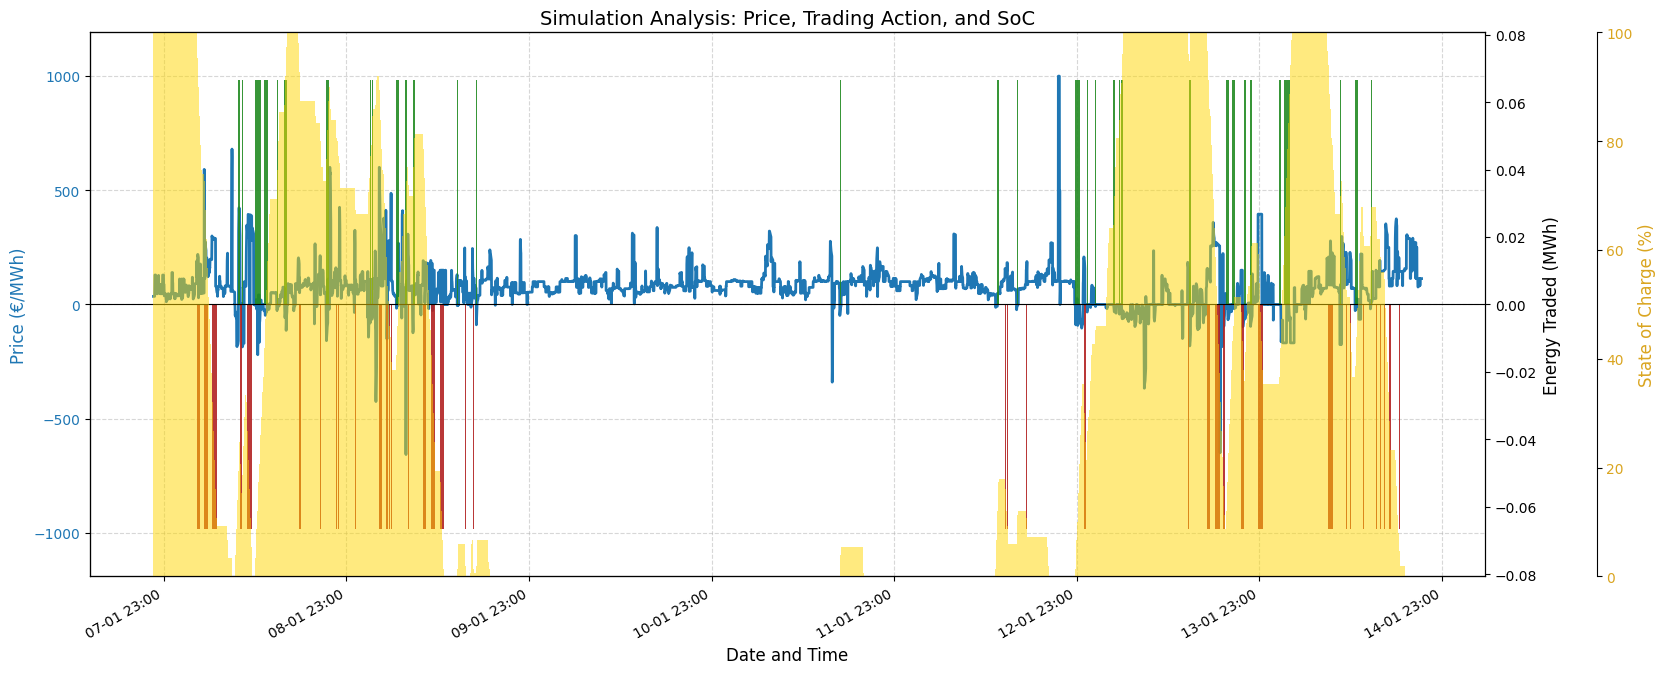
\includegraphics[width=\textwidth]{images/heuristic/no_leverage.png}
                    \caption{Minute-by-minute simulation trace of the heuristic policy.}
                    \label{fig:heuristic_trace}
                \end{figure}

    
        \subsection{Theoretical Upper Bound: The Oracle Policy}
            
            While the heuristic baseline establishes a minimum performance threshold, it is equally important to define a theoretical upper bound. To achieve this, an ``Oracle'' model is introduced. The Oracle operates with perfect foresight, meaning it possesses deterministic knowledge of all future imbalance settlement prices within an evaluation episode. 
            
            The Oracle serves two critical purposes in this research. First, it calculates the absolute maximum revenue achievable, providing a definitive ceiling against which the Reinforcement Learning agents can be measured. Second, it yields a metric for comparing performance across different cross-validation folds. As established in Section \ref{fold-characteristics}, while the $hv$-block splitting ensures seasonal representativeness, the absolute financial opportunity (total market volatility) inherently varies between test sets. By evaluating an agent based on its ratio against the percentage of the Oracle's maximum profit. We can objectively compare algorithmic stability across folds, decoupling the agent's learning efficacy from the arbitrary market volatility of a specific time period.
            
            \subsubsection{Backward Dynamic Programming}
            
            The Oracle computes the optimal trajectory using Backward Dynamic Programming (DP), implemented in Listing \ref{lst:oracle_dp}. The algorithm leverages a key insight into the market mechanics: because the financial settlement is determined solely by the price at the final minute of the 15-minute quarter, the reward within that quarter is strictly linear. Consequently, any mixture of actions within a single quarter is always dominated by a single, continuous 15-minute decision: either fully charge, fully discharge, or remain idle. 
            
            The algorithm operates in two passes:
            \begin{enumerate}
                \item \textbf{Backward Pass:} Starting from the final quarter of the episode with a terminal value of zero, the algorithm works backward in time. For every possible State of Charge (SoC) at every quarter, it evaluates the future value of charging, discharging, or idling, and stores the maximum possible value in a DP table.
                \item \textbf{Forward Pass:} Once the table is populated, the algorithm starts at $t=0$ with an empty battery and traces forward, selecting the exact sequence of actions that yields the maximum cumulative path.
            \end{enumerate}
            
            \begin{listing}[ht]
            \begin{minted}[fontsize=\footnotesize,samepage]{python}
            def compute_oracle_actions(
                prices: np.ndarray,
                battery_capacity: float,
                charge_rate: float,
                cycle_cost: float,
            ):
                """
                Solve for the optimal action per 15-min quarter using backward DP.
                The DP state is (quarter_index, SoC_in_units).
                """
                energy_per_q   = charge_rate * (15 / 60)                          # MWh
                n_soc          = int(round(battery_capacity / energy_per_q)) + 1  # levels
                marginal_cost  = cycle_cost / (2 * battery_capacity)              # EUR/MWh
            
                n_quarters = len(prices) // 15
                settle = np.array([prices[q * 15 + 14] for q in range(n_quarters)])
            
                # Value-to-go and policy tables
                dp     = np.zeros((n_quarters + 1, n_soc))
                policy = np.zeros((n_quarters, n_soc), dtype=int)
            
                # ── Backward pass ──────────────────────────────────────────────────
                for q in range(n_quarters - 1, -1, -1):
                    p = settle[q]
                    for s in range(n_soc):
                        best_val = dp[q + 1, s]          # idle
                        best_a   = 0
            
                        if s + 1 < n_soc:                # charge
                            r = energy_per_q * (-p - marginal_cost)
                            v = r + dp[q + 1, s + 1]
                            if v > best_val:
                                best_val, best_a = v, 1
            
                        if s - 1 >= 0:                   # discharge
                            r = energy_per_q * (p - marginal_cost)
                            v = r + dp[q + 1, s - 1]
                            if v > best_val:
                                best_val, best_a = v, 2
            
                        dp[q, s]     = best_val
                        policy[q, s] = best_a
            
                # ── Forward pass ───────────────────────────────────────────────────
                actions =[]
                soc = 0
                for q in range(n_quarters):
                    a = int(policy[q, soc])
                    actions.append(a)
                    if a == 1:
                        soc += 1
                    elif a == 2:
                        soc -= 1
            
                return actions, float(dp[0, 0])
            \end{minted}
            \caption{Python implementation of the Oracle agent using exact Backward Dynamic Programming to find the optimal trading trajectory.}
            \label{lst:oracle_dp}
            \end{listing}
            
            \subsubsection{Limitations of Exact Dynamic Programming}
            
            This exact mathematical solution is highly efficient for the base model because the state space can be perfectly discretized. Given a 10 MW capacity and a 5 MW charge rate, a 15-minute action corresponds exactly to a 1.25 MWh step in SoC. This creates a strictly bounded, 1-dimensional grid of exactly 9 possible SoC states, resulting in zero approximation error.
            
            However, this tabular DP approach is rigid. As the complexity of the physical environment increases, exact DP quickly becomes computationally intractable or mathematically impossible. If the model is extended to include continuous action spaces (e.g., modulating power output minute-by-minute), non-linear battery degradation (where wear depends dynamically on depth-of-discharge), or round-trip efficiency losses that decouple traded energy from physically stored energy, the state space explodes. This phenomenon, known as the \textit{curse of dimensionality}, renders perfect foresight solvers infeasible. It is precisely this limitation of traditional optimization that necessitates the use of Deep Reinforcement Learning.

            \subsubsection{Performance Evaluation}
                To establish the absolute ceiling for the reinforcement learning agents, the Oracle model was executed across the test sets of all five $hv$-block cross-validation folds. The theoretical maximum net revenues achievable with perfect foresight are detailed in Table \ref{tab:oracle_results}.
                
                \begin{table}[h]
                    \centering
                    \renewcommand{\arraystretch}{1.2} 
                    \begin{tabular}{c r}
                        \hline
                        \textbf{Cross-Validation Fold} & \textbf{Theoretical Max Revenue (Euro (€))} \\
                        \hline
                        Fold 0 & 852,584.75 \\
                        Fold 1 & 802,363.82 \\
                        Fold 2 & 817,079.34 \\
                        Fold 3 & 814,775.11 \\
                        Fold 4 & 833,643.13 \\
                        \hline
                        \textbf{Mean $\pm$ Std. Dev.} & \textbf{824,089.23 $\pm$ 19,250.45} \\
                        \hline
                    \end{tabular}
                    \caption{Theoretical maximum net revenue per fold, calculated by the Oracle model using exact backward dynamic programming.}
                    \label{tab:oracle_results}
                \end{table}
                
                Beyond providing the baseline for the Optimality Ratio, the results in Table \ref{tab:oracle_results} serve a secondary, highly valuable methodological purpose: they act as a financial validation of the data partitioning strategy. 
                
                Because the Oracle extracts the absolute maximum value available in the market, its performance is a direct measure of the total ``market opportunity'' present within a specific dataset. If the data splitting had been performed poorly—for instance, if Fold 0 inadvertently contained a disproportionate amount of highly volatile winter crises while Fold 1 contained only stagnant summer weeks—the Oracle's revenue would fluctuate wildly between the folds. 
                
                However, the results demonstrate remarkable consistency. Across all five folds, the maximum theoretical revenue remains tightly clustered around a mean of 824,089€, with a standard deviation of less than 2.5\%. This financial homogeneity confirms that every single test fold contains a nearly identical distribution of arbitrage opportunities and market volatility. Consequently, this provides a powerful, empirical reassurance that the systematic interleaving of the $hv$-block cross-validation successfully stratified the seasonal non-stationarity of the dataset, ensuring a perfectly fair and balanced evaluation landscape for the reinforcement learning agents.
                            

        \subsection{Algorithmic Benchmarking and Policy Selection}
            
            Having established the theoretical upper bound via the Oracle model, the analysis now turns to evaluating the performance of the selected Deep Reinforcement Learning agents. Before examining the individual algorithmic results, it is critical to outline the statistical methodology used to decouple the different sources of variance inherent in this evaluation.
            
            \subsubsection{Methodology: Deconstructing Variance}
            
            Evaluating a DRL algorithm on a single test run, or even a single pass over cross-validation folds, provides an incomplete picture of its true capabilities. The final performance of an agent is heavily influenced by data variance and algorithmic variance.
            
            If a model is only trained once per fold, the resulting standard deviation across the $K$ folds solely measures data variance this is how well the agent handles different market regimes (e.g., winter vs. summer). However, this metric completely obscures algorithmic variance. DRL algorithms are highly sensitive to stochastic weight initialization, random exploratory actions taken early in training, and the random sampling of batches from experience replay buffers. Consequently, two identical agents trained on the exact same fold can converge to vastly different policies simply due to a lucky or unlucky random seed.
            
            To isolate these effects, our evaluation framework employs a two-tiered statistical approach. For every $hv$-block cross-validation fold, the agent is trained from scratch $N$ independent times (using different random seeds). This allows us to measure:
            \begin{enumerate}
                \item \textbf{Intra-Fold Standard Deviation (Algorithmic Stability):} The variance in performance across the $N$ independent runs \textit{within the same fold}. A high intra-fold variance indicates that the algorithm is unstable and highly dependent on lucky initializations.
                \item \textbf{Cross-Fold Standard Deviation (Market Robustness):} The variance of the mean performance \textit{across the $K$ different folds}. A high cross-fold variance indicates that the agent struggles to generalize to different market conditions.
            \end{enumerate}
            By separating these metrics, we can definitively diagnose whether poor performance is due to an inability to handle the specific market data, or an inherent instability in the learning algorithm itself.
            
           \subsubsection{Deep Q-Network (DQN) Performance Evaluation}
                        
            The first agent evaluated is the Deep Q-Network (DQN) \cite{mnih2013playing}. To understand the architecture of DQN, it is essential to first outline the mathematical foundations of classical Q-learning from which it is derived. 
            
            \paragraph{The Foundations: Q-Learning and the Bellman Equation}
            As a value-based method, the objective of Q-learning is to find the optimal action-value function, denoted as $Q^*(S_t, A_t)$. This function calculates the expected cumulative discounted reward of taking action $A_t$ in state $S_t$, assuming that the agent acts optimally in all subsequent steps. According to the Bellman optimality equation, this value can be decomposed into two parts: the immediate reward received, and the discounted optimal value of the state that follows:
            \[
                Q^*(S_t, A_t) = \mathbb{E} \left[ R_{t+1} + \gamma \max_{a} Q^*(S_{t+1}, a) \right]
            \]
            
            Traditional Q-learning solves this equation iteratively using Temporal Difference (TD) learning. Instead of waiting until the end of an episode to calculate the total reward, the agent updates its value estimations step-by-step. It stores every state-action pair in a large matrix (a Q-table) and continuously refines these values through a cycle of interaction and learning.
            
            \paragraph{Action Selection: The Exploration-Exploitation Trade-off}
            Before the agent can update its Q-values, it must first interact with the environment by selecting an action $A_t$ in the current state $S_t$. To accurately populate the Q-table, the agent must gather diverse experiences. This requires a delicate balance between \textit{exploitation} (choosing the action with the highest currently known Q-value to maximize immediate profit) and \textit{exploration} (choosing random actions to discover potentially superior, unmapped strategies). 
            
            This decision process is governed by an $\epsilon$-greedy policy. Under this policy, the agent generates a random number between 0 and 1. If the number is less than a threshold $\epsilon$, the agent explores by selecting a purely random action from the action space. Otherwise, it exploits its current knowledge by selecting $\arg\max_a Q(S_t, a)$. At the start of training, $\epsilon$ is set high (e.g., 0.99), forcing the agent to explore the market extensively. Over time, the value of $\epsilon$ systematically decays, because the table will already be filled in with the higher values.
            
            \paragraph{The Value Update}
            Once the action $A_t$ is executed (whether chosen via exploration or exploitation), the environment transitions to a new state $S_{t+1}$ and yields an immediate reward $R_{t+1}$. The agent then updates its Q-table using the following rule:
            \[
                Q(S_t, A_t) \leftarrow Q(S_t, A_t) + \alpha \left[ R_{t+1} + \gamma \max_{a} Q(S_{t+1}, a) - Q(S_t, A_t) \right]
            \]
            
            This fundamental update equation consists of several distinct components; this is also clarified further in Figure \ref{fig:q-learning-action-value-update}:
            \begin{itemize}
                \item $Q(S_t, A_t)$: The former Q-value estimation for the specific state-action pair just experienced.
                \item $\alpha \in [0, 1]$: The learning rate, which dictates how aggressively new information overrides old information.
                \item $R_{t+1} + \gamma \max_{a} Q(S_{t+1}, a)$: This term is the \textbf{TD Target}. It is the sum of the immediate reward ($R_{t+1}$) and the discounted estimate of the optimal Q-value for the next state.
                \item The entire term inside the brackets is the \textbf{TD Error}. It calculates the mathematical difference between the agent's new target and its former estimation.
            \end{itemize}
            
            % TODO reference website? (e.g., adapted from Hugging Face Deep RL Course)
            \begin{figure}[h]
                \centering
                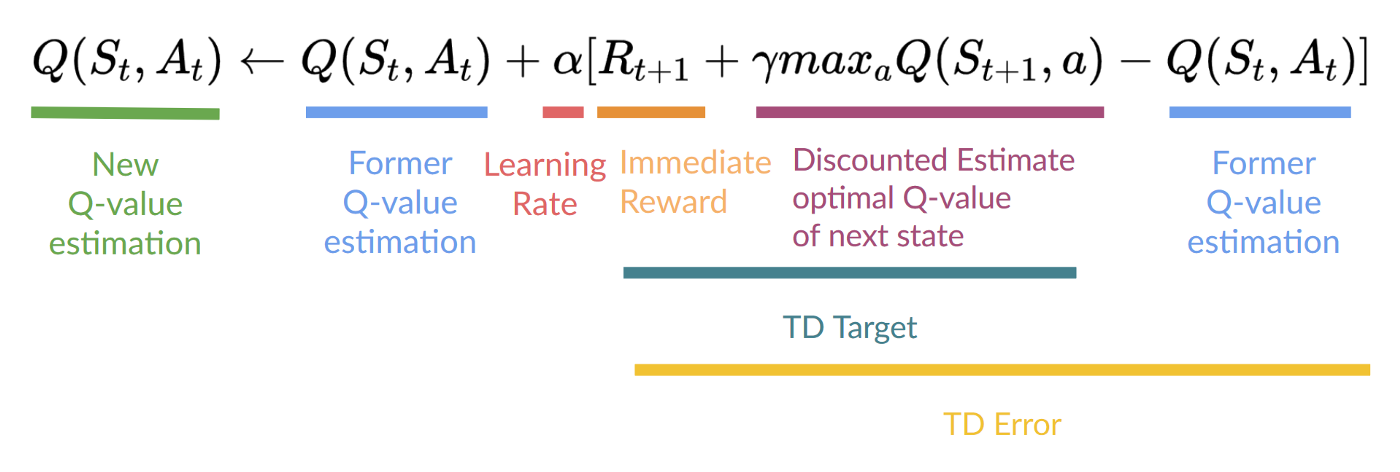
\includegraphics[width=\textwidth]{images/Q-learning-theory/Q-learning-8.jpg}
                \caption{Visual breakdown of the Q-learning state-action value function update equation.}
                \label{fig:q-learning-action-value-update}
            \end{figure}
            
            \paragraph{From Tabular Q-Learning to Deep Q-Networks}
            While traditional tabular Q-learning is mathematically sound, it suffers from a fatal flaw in complex environments: maintaining a discrete table for every possible state-action pair becomes computationally impossible when the state space contains continuous variables. The nature of electricity prices and the highly granular State of Charge (SoC) create a practically infinite number of states.
                        
            DQN resolves this curse of dimensionality by eliminating the Q-table entirely and replacing it with a deep neural network (a Multi-Layer Perceptron) acting as a non-linear function approximator, parameterized by weights $\theta$. The network takes the continuous state vector $S_t$ as input and outputs the estimated Q-values for all discrete actions simultaneously. The agent learns by minimizing the Mean Squared Error (MSE) of the Temporal Difference (TD) error via gradient descent. 
            
            However, introducing a non-linear function approximator into reinforcement learning typically causes severe training instability due to highly correlated sequential observations and constantly shifting optimization targets. To ensure mathematical convergence, the DQN architecture relies on three critical stabilizing mechanisms \cite{mnih2015humanlevel}:
            \begin{enumerate}
                \item \textbf{Experience Replay:} Transitions $e_t = (S_t, A_t, R_{t+1}, S_{t+1})$ are stored in a cyclic Replay Buffer. The network is updated using randomized mini-batches sampled from this buffer, breaking temporal autocorrelation and satisfying the i.i.d. assumption required for gradient descent.
                \item \textbf{Fixed Q-Targets:} To prevent the learning target from shifting at every step, DQN utilizes a secondary, frozen \textit{Target Network} ($\theta^-$) to calculate the TD Target: $R_{t+1} + \gamma \max_{a} Q(S_{t+1}, a; \theta^-)$. The weights $\theta^-$ are only synchronized with the main policy network at fixed intervals.
                \item \textbf{$\epsilon$-Greedy Exploration:} The same mechanism as in tabular Q-learning. A scheduled decay that forces the agent to take random actions early in training to map the state space, gradually shifting toward deterministic exploitation ($\pi(S_t) = \arg\max_a Q(S_t, a; \theta)$) as the network matures.
            \end{enumerate}
            
            \paragraph{Performance and Variance Analysis}
            The practical impact of these architectural mechanisms is distinctly visible in the agent's empirical performance. The learning trajectory across the training horizon is visualized in Figure \ref{fig:dqn_per_fold}, with the corresponding variance analysis detailed in Figure \ref{fig:dqn_variance}.
            
            \begin{figure}[htbp]
                \centering
                \begin{minipage}{0.48\textwidth}
                    \centering
                    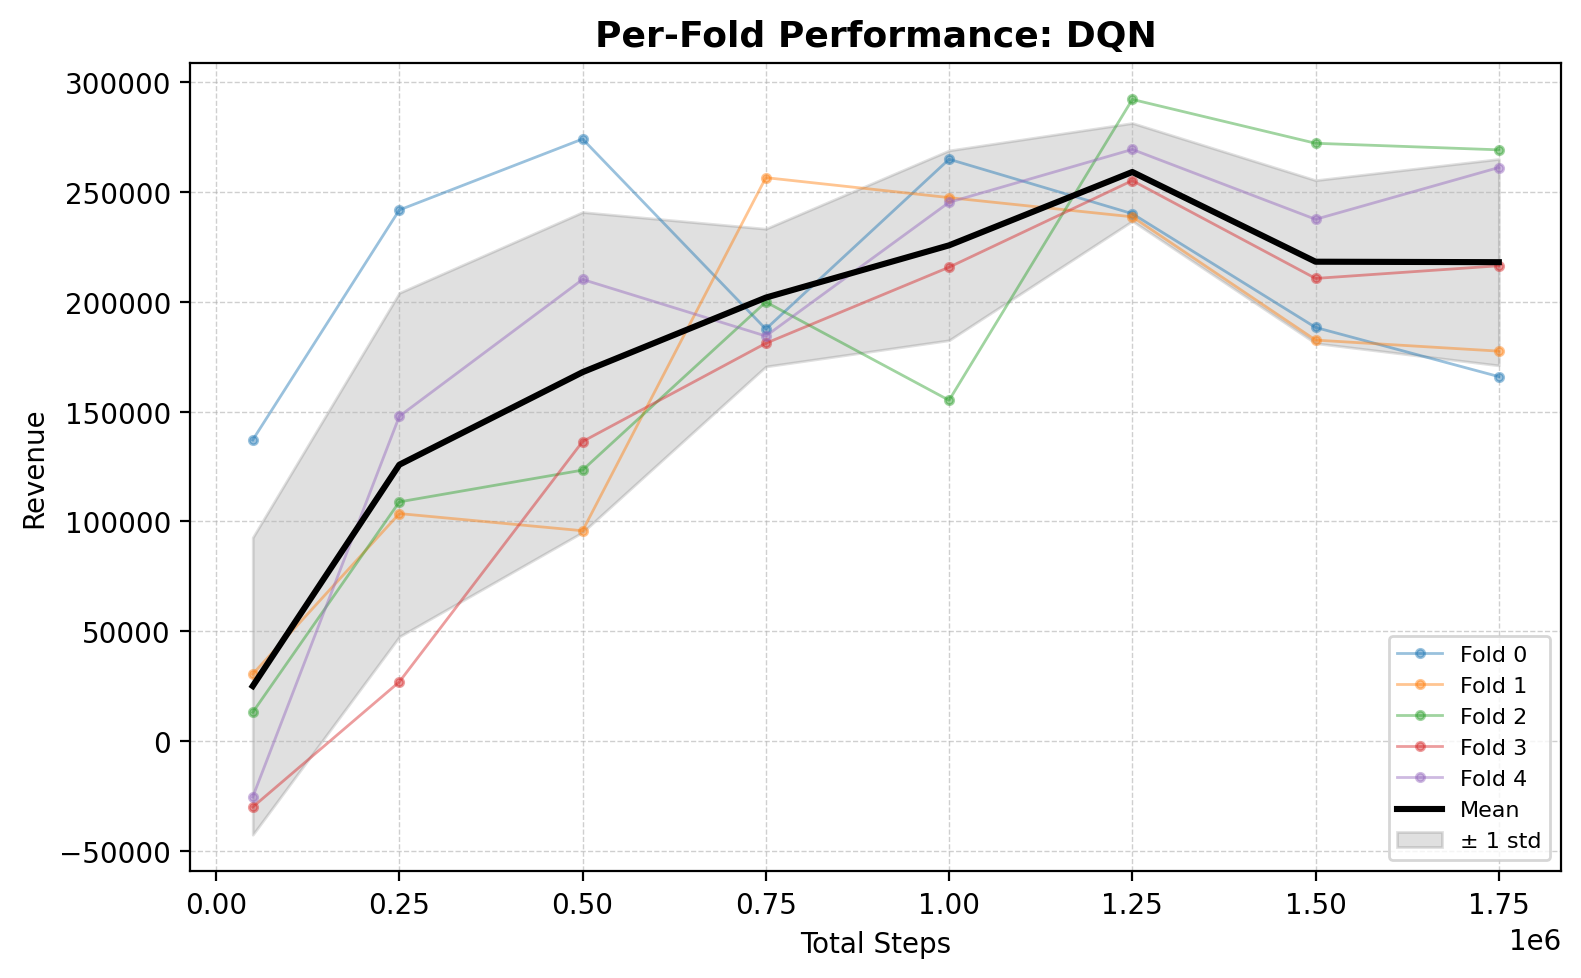
\includegraphics[width=\linewidth]{images/agent-evaluation/agent_per_fold_DQN.png}
                    \caption{Per-fold learning curves for the DQN agent, illustrating the mean net revenue and $\pm 1$ standard deviation across independent training runs.}
                    \label{fig:dqn_per_fold}
                \end{minipage}\hfill
                \begin{minipage}{0.48\textwidth}
                    \centering
                    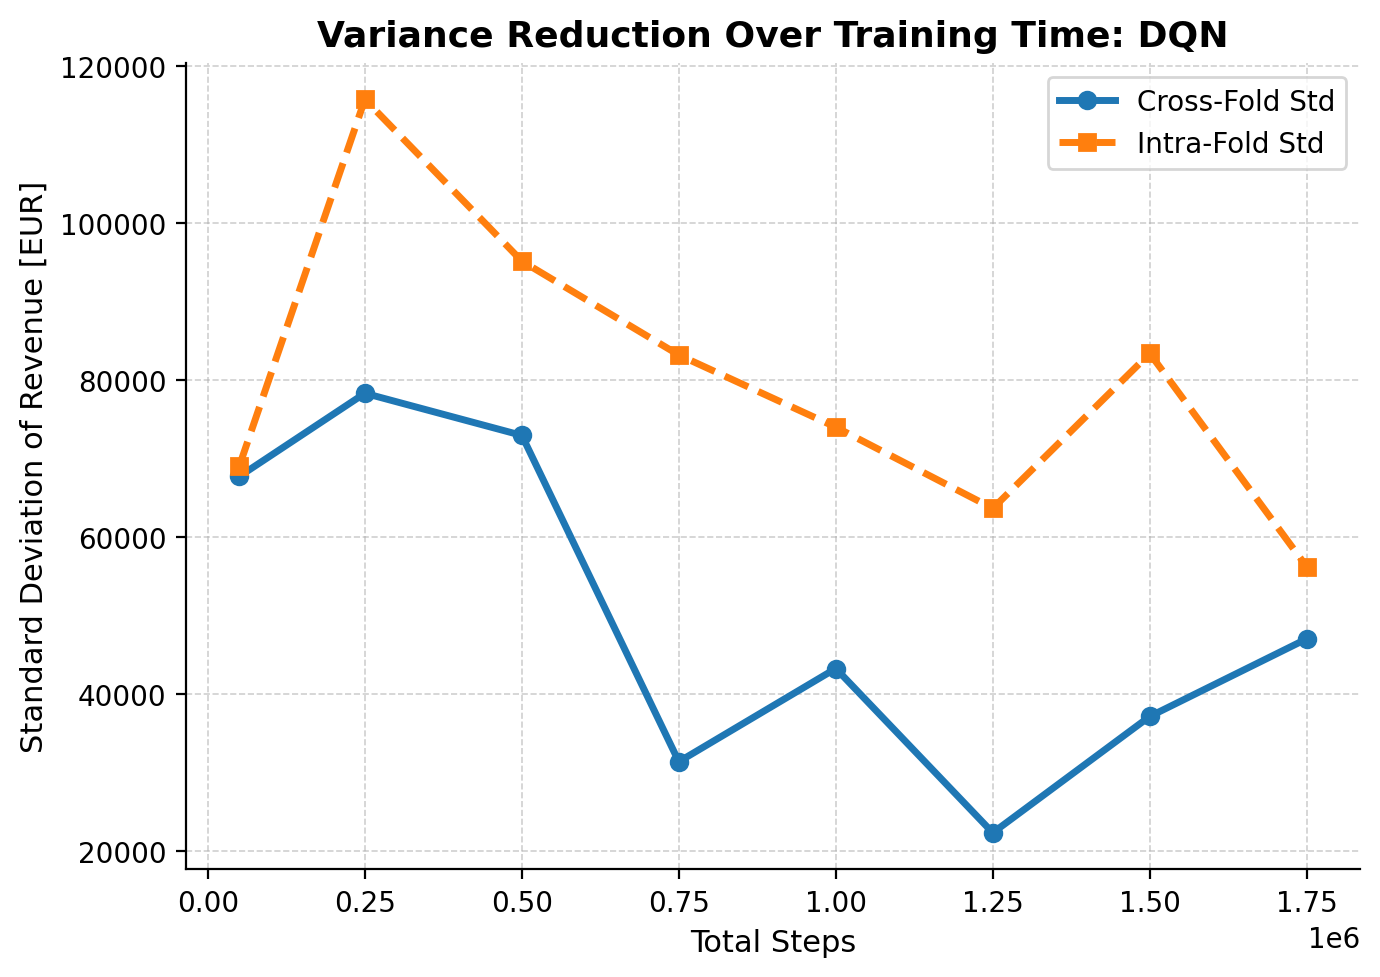
\includegraphics[width=\linewidth]{images/agent-evaluation/variance_over_time_DQN.png}
                    \caption{Comparison of Intra-Fold (Algorithmic) and Cross-Fold (Market) standard deviation for the DQN agent over the training horizon.}
                    \label{fig:dqn_variance}
                \end{minipage}
            \end{figure}
            
            As observed in Figure \ref{fig:dqn_per_fold}, the initial performance of the DQN agent is exceptionally poor, occasionally yielding negative net revenue. A steady improvement occurs as training progresses, with the mean revenue peaking near 1.25 million steps. However, Figure \ref{fig:dqn_variance} reveals a massive initial spike in \textbf{Intra-Fold Standard Deviation} that only steadily degrades as the agent is given more training steps. 
            
            This specific learning dynamic—high initial volatility followed by pronounced stabilization—is a direct reflection of DQN's stabilizing mechanisms maturing over time:
            \begin{itemize}
                \item \textbf{Buffer Saturation:} Early in training, the Experience Replay buffer is either sparse or filled with low-quality, random exploratory transitions. Consequently, the mini-batches sampled for gradient descent are highly volatile, leading to chaotic policy updates and massive algorithmic variance between independent runs. As training steps increase, the buffer becomes saturated with more representative rewards and transitions, smoothing the gradient updates and driving the intra-fold variance down.
                
                TODO Quesiton! -> Relevant to support this with a graph on mean reward in experience buffer? So how the mean increasing?  
                
                \item \textbf{Exploration Decay:} In the early stages, high $\epsilon$ values force the agent into highly stochastic behavior. Because these random exploratory actions differ based on the initialization seed of each run, the intra-fold variance is inherently large. As $\epsilon$ decays toward its minimum bound, the agent shifts into deterministic exploitation, which directly correlates with the observed rise in revenue and the sharp drop in algorithmic variance.
                \item \textbf{Target Convergence:} Initially, the Q-values are wildly inaccurate, meaning the periodic synchronizations to the Target Network cause disruptive shifts in the policy landscape. Over millions of steps, as the primary Q-network begins to converge on the true value function, these target updates become less jarring, further stabilizing the learning curve.
            \end{itemize}
            
            Despite this eventual stabilization, the peak absolute revenue remains significantly below the Oracle's theoretical maximum. Ultimately, DQN struggles to master the complex leverage required for optimal battery arbitrage.
             \subsubsection{Proximal Policy Optimization (PPO) Performance Evaluation}

            The second agent evaluated is Proximal Policy Optimization (PPO) \cite{schulman2017proximal}. PPO belongs to a fundamentally different family of reinforcement learning algorithms than DQN. Rather than learning a Q-function and deriving a policy from it (value-based), PPO is a policy gradient method: it directly parameterizes and optimizes the policy $\pi_\theta$ itself.

            \paragraph{The Foundations: Policy Gradient Methods}
            Instead of asking ``what is the value of this state-action pair?'', policy gradient methods ask: ``how should I adjust the parameters $\theta$ of my policy to make profitable actions more likely?'' The objective is to maximize the expected cumulative reward directly:
            \[
                J(\theta) = \mathbb{E}_{\pi_\theta} \left[ \sum_{t=0}^{T} \gamma^t R(S_t, x_t) \right]
            \]
            The policy gradient theorem provides the gradient of this objective with respect to the policy parameters:
            \[
                \nabla_\theta J(\theta) = \mathbb{E}_{\pi_\theta} \left[ \nabla_\theta \log \pi_\theta(x_t \mid S_t) \cdot G_t \right]
            \]
            where $G_t$ is the return from time $t$ onwards. Intuitively, this rule increases the log-probability of actions that led to high returns and decreases it for actions that led to low returns.

            \paragraph{The Actor-Critic Architecture}
            A practical challenge with pure policy gradient methods is the high variance of the gradient estimate. Using the raw return $G_t$ as a learning signal is noisy, as a single bad episode can push the policy in entirely the wrong direction. PPO addresses this by adopting an Actor-Critic architecture, which maintains two separate neural networks:
            \begin{itemize}
                \item \textbf{Actor ($\pi_\theta$):} The policy network. It maps the current state $S_t$ to a probability distribution over the discrete action space, selecting which action $x_t$ to execute.
                \item \textbf{Critic ($V_\phi$):} The value network. It maps the state $S_t$ to a scalar estimate of the expected future return from that state, $\hat{V}(S_t)$.
            \end{itemize}
            The critic's estimate is used to compute the \textit{Advantage} $\hat{A}_t$, which measures how much better or worse the taken action was compared to the average action in that state:
            \[
                \hat{A}_t = G_t - \hat{V}(S_t)
            \]
            Replacing the raw return $G_t$ with the advantage $\hat{A}_t$ in the gradient update dramatically reduces variance, as the critic subtracts the estimated value of simply being in state $S_t$.

            \paragraph{The Core PPO Mechanism: The Clipped Surrogate Objective}
            The defining contribution of PPO is a principled solution to a fundamental instability in policy gradient training. When the gradient step is too large, the new policy can diverge catastrophically from the old one, causing performance to collapse irreversibly. PPO prevents this by introducing the \textit{clipped surrogate objective}. Let $r_t(\theta)$ denote the probability ratio between the updated policy and the policy that collected the data:
            \[
                r_t(\theta) = \frac{\pi_\theta(x_t \mid S_t)}{\pi_{\theta_{\text{old}}}(x_t \mid S_t)}
            \]

            \begin{itemize}
                \item if $r_t(\theta) > 1$ the action $a_t$ at state $s_t$ is more likely in the current policy than the old policy.
                \item if $r_t(\theta)$ is between 0 and 1, the action is less likely for the current policy than for the old one.
            \end{itemize}
            
            PPO clips this ratio to lie within a small interval $[1 - \varepsilon, 1 + \varepsilon]$, where $\varepsilon$ is a hyperparameter (typically 0.2):
            \[
                \mathcal{L}^{\text{CLIP}}(\theta) = \mathbb{E}_t \left[ \min \left( r_t(\theta)\,\hat{A}_t,\; \text{clip}(r_t(\theta),\, 1-\varepsilon,\, 1+\varepsilon)\,\hat{A}_t \right) \right]
            \]
            This objective acts as a conservative trust region: if an update would move the policy too far from its previous version, the gradient is zeroed out at the clip boundary. It results in monotonically improving updates.
            
            The result is a ``little-but-often'' learning approach that makes safe, monotonically improving updates rather than risky large leaps.

            % TODO reference website? (e.g., adapted from Hugging Face Deep RL Course)
            \begin{figure}[h]
                \centering
                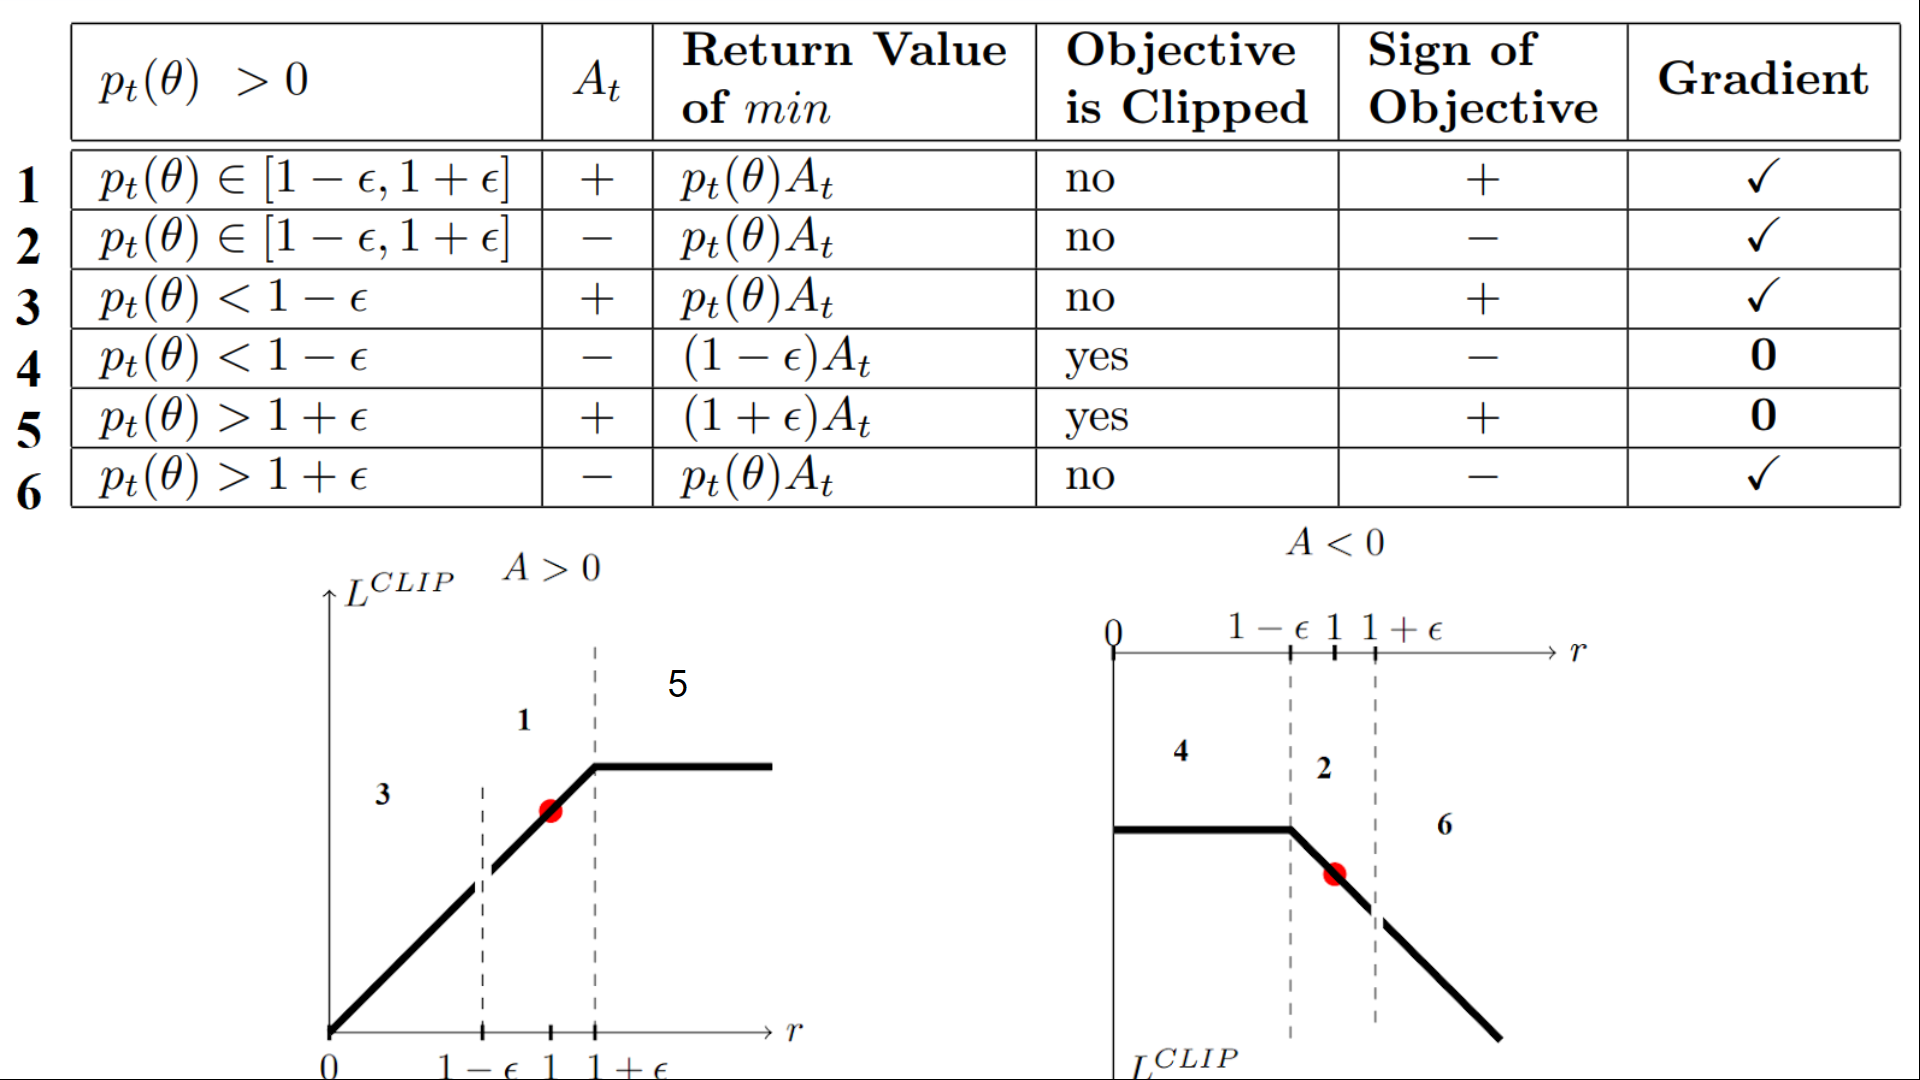
\includegraphics[width=\textwidth]{images/Q-learning-theory/table-ppo.png}
                \caption{Visual breakdown clipping procedure in PPO}
                \label{fig:ppo-clipping}
            \end{figure}

            \paragraph{On-Policy Data Collection and Entropy Regularization}
            PPO is an on-policy algorithm: it collects a fresh batch of transitions using its current policy, performs several gradient update epochs on that batch, and then discards it. This keeps the training distribution aligned with the current policy at all times; it is perhaps because of this that we see a faster rise in revenue compared to DQN. DQN looks at it's replay buffer, which in the early stages is not yet filled up with representative values.

            To maintain sufficient exploration throughout training, PPO augments the objective with an entropy bonus $\mathcal{H}[\pi_\theta(\cdot \mid S_t)]$. By penalizing an overly deterministic policy, the agent is encouraged to remain curious, discovering leverage strategies rather than prematurely committing to a suboptimal policy.

            \paragraph{Performance and Variance Analysis}
            The practical consequence of these architectural choices is immediately evident in the agent's empirical performance. The learning trajectory is visualized in Figure \ref{fig:ppo_per_fold}, with the corresponding variance analysis in Figure \ref{fig:ppo_variance}.

            \begin{figure}[htbp]
                \centering
                \begin{minipage}{0.48\textwidth}
                    \centering
                    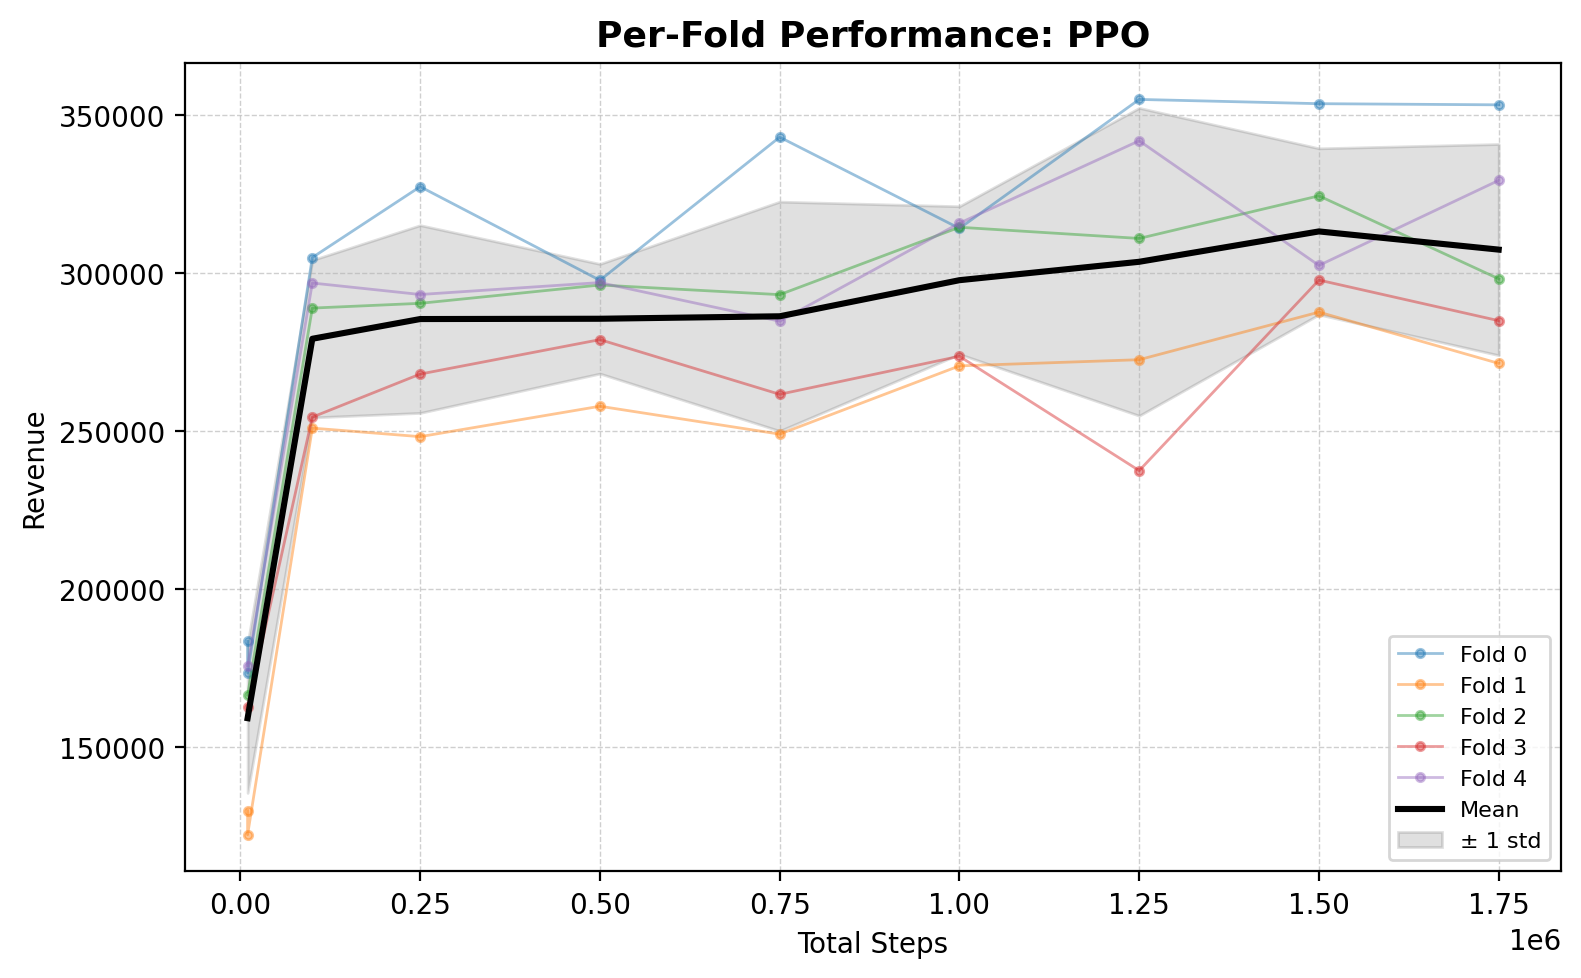
\includegraphics[width=\linewidth]{images/agent-evaluation/agent_per_fold_PPO.png}
                    \caption{Per-fold learning curves for the PPO agent, illustrating the mean net revenue and $\pm 1$ standard deviation across independent training runs.}
                    \label{fig:ppo_per_fold}
                \end{minipage}\hfill
                \begin{minipage}{0.48\textwidth}
                    \centering
                    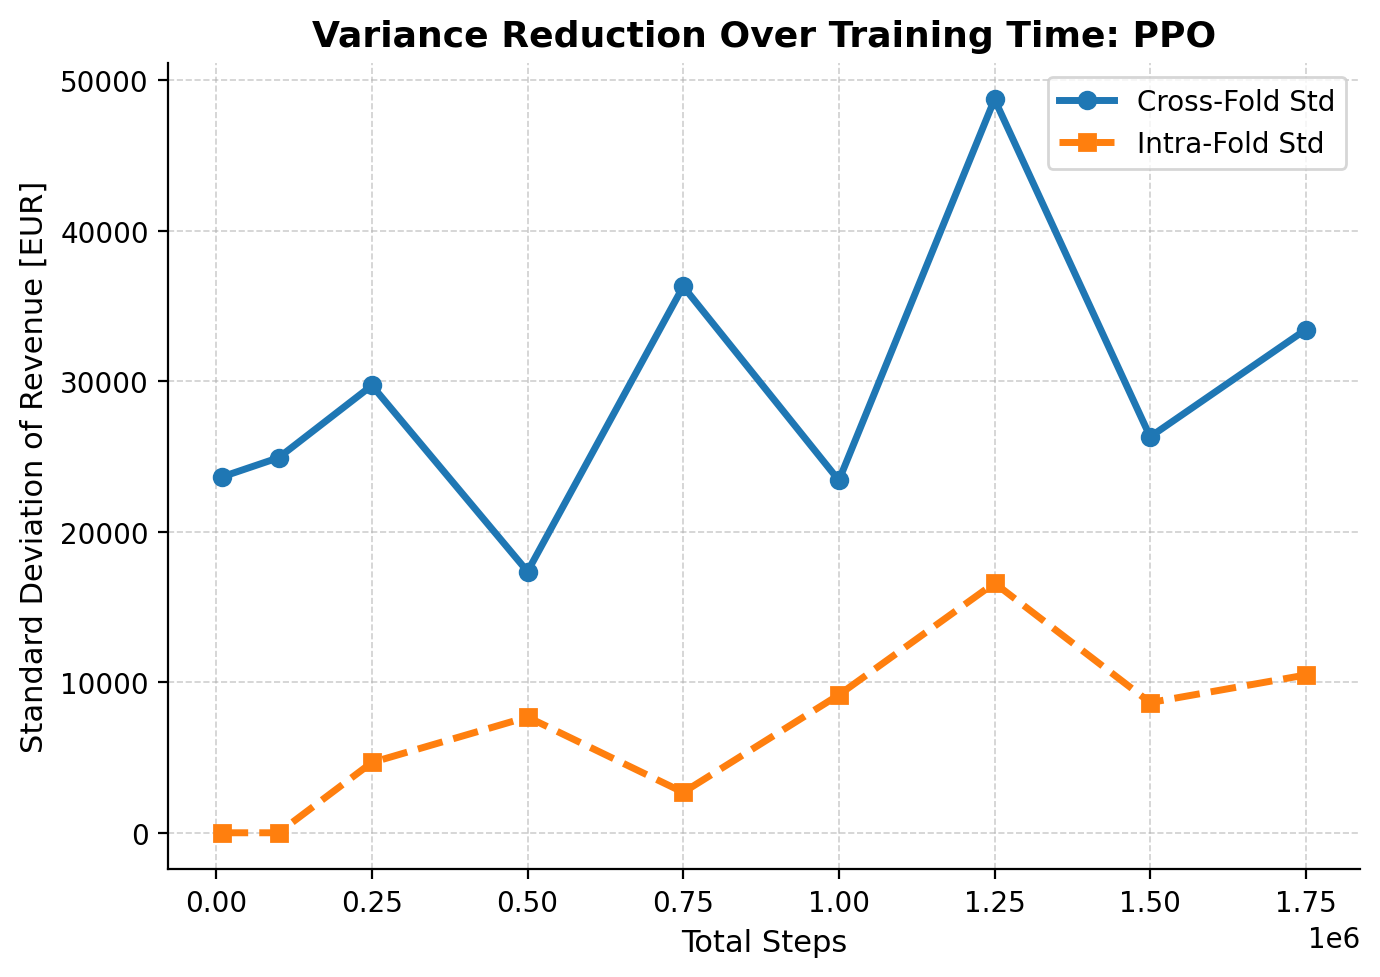
\includegraphics[width=\linewidth]{images/agent-evaluation/variance_over_time_PPO.png}
                    \caption{Comparison of Intra-Fold (Algorithmic) and Cross-Fold (Market) standard deviation for the PPO agent over the training horizon.}
                    \label{fig:ppo_variance}
                \end{minipage}
            \end{figure}

            In stark contrast to DQN, PPO converges to it's plateau revenue in a fraction of the training steps. with the mean performance across folds remaining tightly aligned throughout. Crucially, Figure \ref{fig:ppo_variance} reveals a small Intra-Fold Standard Deviation throughout the training, indicating that different random seeds reliably converge to the same policy.

            Each architectural choice contributes directly to this observed stability:
            \begin{itemize}
                \item \textbf{Clipping eliminates catastrophic updates:} Where DQN's early training is destabilized by rapidly shifting Q-targets, PPO's clipped objective enforces a hard constraint on the size of each policy update. No single bad batch can send the policy into an irrecoverable collapse, which is why the intra-fold variance never spikes as observed with DQN.
                \item \textbf{Advantage normalization reduces gradient noise:} By subtracting the critic's value baseline, the advantage estimate $\hat{A}_t$ centers the learning signal around zero. This makes gradient updates far less sensitive to the scale of absolute rewards, which in the imbalance market can range rather greatly.
                \item \textbf{On-policy freshness accelerates convergence:} Because every training batch is generated by the current policy, the actor and critic are always trained on data that reflects their current behavior. This direct feedback loop allows the policy to more quickly identify better values.
            \end{itemize}


            \subsubsection{Soft Actor-Critic (SAC) Performance Evaluation}

            The third agent evaluated is Soft Actor-Critic (SAC) \cite{haarnoja2018soft}. SAC is an off-policy algorithm, meaning it can reuse past experience similarly to DQN, while simultaneously maintaining the actor-critic structure of PPO. However, its defining characteristic is a fundamentally different learning objective: rather than simply maximizing expected cumulative reward, SAC maximises a trade-off between reward and the \textit{entropy} of the policy.

            \paragraph{The Maximum Entropy Framework}
            Classical reinforcement learning seeks a policy that maximises the discounted return:
            \[
                J(\theta) = \mathbb{E}_{\pi_\theta} \left[ \sum_{t=0}^{T} \gamma^t R(S_t, x_t) \right]
            \]
            SAC augments this objective with a weighted entropy term at every time step:
            \[
                J_{\text{SAC}}(\theta) = \mathbb{E}_{\pi_\theta} \left[ \sum_{t=0}^{T} \gamma^t \Bigl( R(S_t, x_t) + \alpha \,\mathcal{H}\bigl[\pi_\theta(\cdot \mid S_t)\bigr] \Bigr) \right]
            \]
            where $\mathcal{H}[\pi_\theta(\cdot \mid S_t)] = -\sum_a \pi_\theta(a \mid S_t)\log \pi_\theta(a \mid S_t)$ is the Shannon entropy of the policy in state $S_t$, and $\alpha > 0$ is the \textit{temperature} parameter that controls the relative importance of the entropy term versus the reward signal.

            The practical effect of this augmentation is that the agent is explicitly rewarded for remaining uncertain. A policy that spreads probability mass over multiple actions receives a bonus, whereas a policy that commits deterministically to one action forfeits that bonus. This built-in incentive to explore prevents premature convergence to a locally profitable but globally suboptimal strategy, a characteristic risk in highly non-stationary markets such as the Belgian imbalance market.

            \paragraph{Soft Bellman Equations and Dual Q-Networks}
            The maximum entropy objective requires a revised set of Bellman equations. The soft Q-function now satisfies:
            \[
                Q_{\text{soft}}(S_t, x_t) = R(S_t, x_t) + \gamma\, \mathbb{E}_{S_{t+1}} \Bigl[ V_{\text{soft}}(S_{t+1}) \Bigr]
            \]
            \[
                V_{\text{soft}}(S_t) = \mathbb{E}_{x_t \sim \pi_\theta} \Bigl[ Q_{\text{soft}}(S_t, x_t) - \alpha \log \pi_\theta(x_t \mid S_t) \Bigr]
            \]
            The soft value function $V_{\text{soft}}$ integrates both the expected future Q-value \textit{and} the entropy of the current policy. A high-entropy state---one in which the agent sees multiple promising actions---is therefore intrinsically valuable, even before any reward is collected.

            In practice, SAC maintains \textbf{two independent critic networks} $Q_{\phi_1}$ and $Q_{\phi_2}$, both trained on data sampled from a shared experience replay buffer. When computing the TD target, the minimum of the two critics is used:
            \[
                y = R_{t+1} + \gamma \Bigl( \min_{i=1,2} Q_{\phi_i}(S_{t+1}, x_{t+1}) - \alpha \log \pi_\theta(x_{t+1} \mid S_{t+1}) \Bigr)
            \]
            This \textit{clipped double-Q} trick directly counteracts the well-known \textit{overestimation bias} that plagues single-critic value-based methods. By always taking the pessimistic estimate of the two critics, SAC avoids chasing inflated Q-values that would otherwise cause unstable or greedy policies.

            \paragraph{Automatic Entropy Tuning}
            A key practical contribution of the SAC framework is the automatic adjustment of the temperature $\alpha$. Rather than treating it as a fixed hyperparameter, SAC casts the temperature as the solution to the following constrained optimisation problem:
            \[
                \alpha^* = \arg\min_\alpha\; \mathbb{E}_{x_t \sim \pi_{\theta^*}} \Bigl[ -\alpha \log \pi_{\theta^*}(x_t \mid S_t) - \alpha \bar{\mathcal{H}} \Bigr]
            \]
            where $\bar{\mathcal{H}}$ is a minimum target entropy (typically set to $-|\mathcal{A}|$). If the policy becomes too deterministic (entropy falls below $\bar{\mathcal{H}}$), $\alpha$ increases to encourage further exploration. Conversely, once the agent has found a reliable strategy and entropy already exceeds the target, $\alpha$ decreases to allow confident exploitation. This self-regulating mechanism eliminates tedious manual temperature tuning and makes SAC considerably more robust to new market regimes encountered across different cross-validation folds.

            \paragraph{Off-Policy Data Collection}
            Like DQN, SAC is an \textit{off-policy} algorithm: transitions $(S_t, x_t, R_{t+1}, S_{t+1})$ are stored in a large replay buffer and sampled in randomised mini-batches for every gradient update. This decouples the frequency of data collection from the frequency of learning, making SAC substantially more \textit{sample efficient} than the on-policy PPO. A single market episode can contribute to many gradient updates, amortising the cost of environmental interaction. In a setting where live data collection is expensive or time-consuming, this is a significant practical advantage.

            \paragraph{Performance and Variance Analysis}
            The empirical performance of SAC is presented in Figure \ref{fig:sac_per_fold}, and the accompanying variance decomposition in Figure \ref{fig:sac_variance}.

            \begin{figure}[htbp]
                \centering
                \begin{minipage}{0.48\textwidth}
                    \centering
                    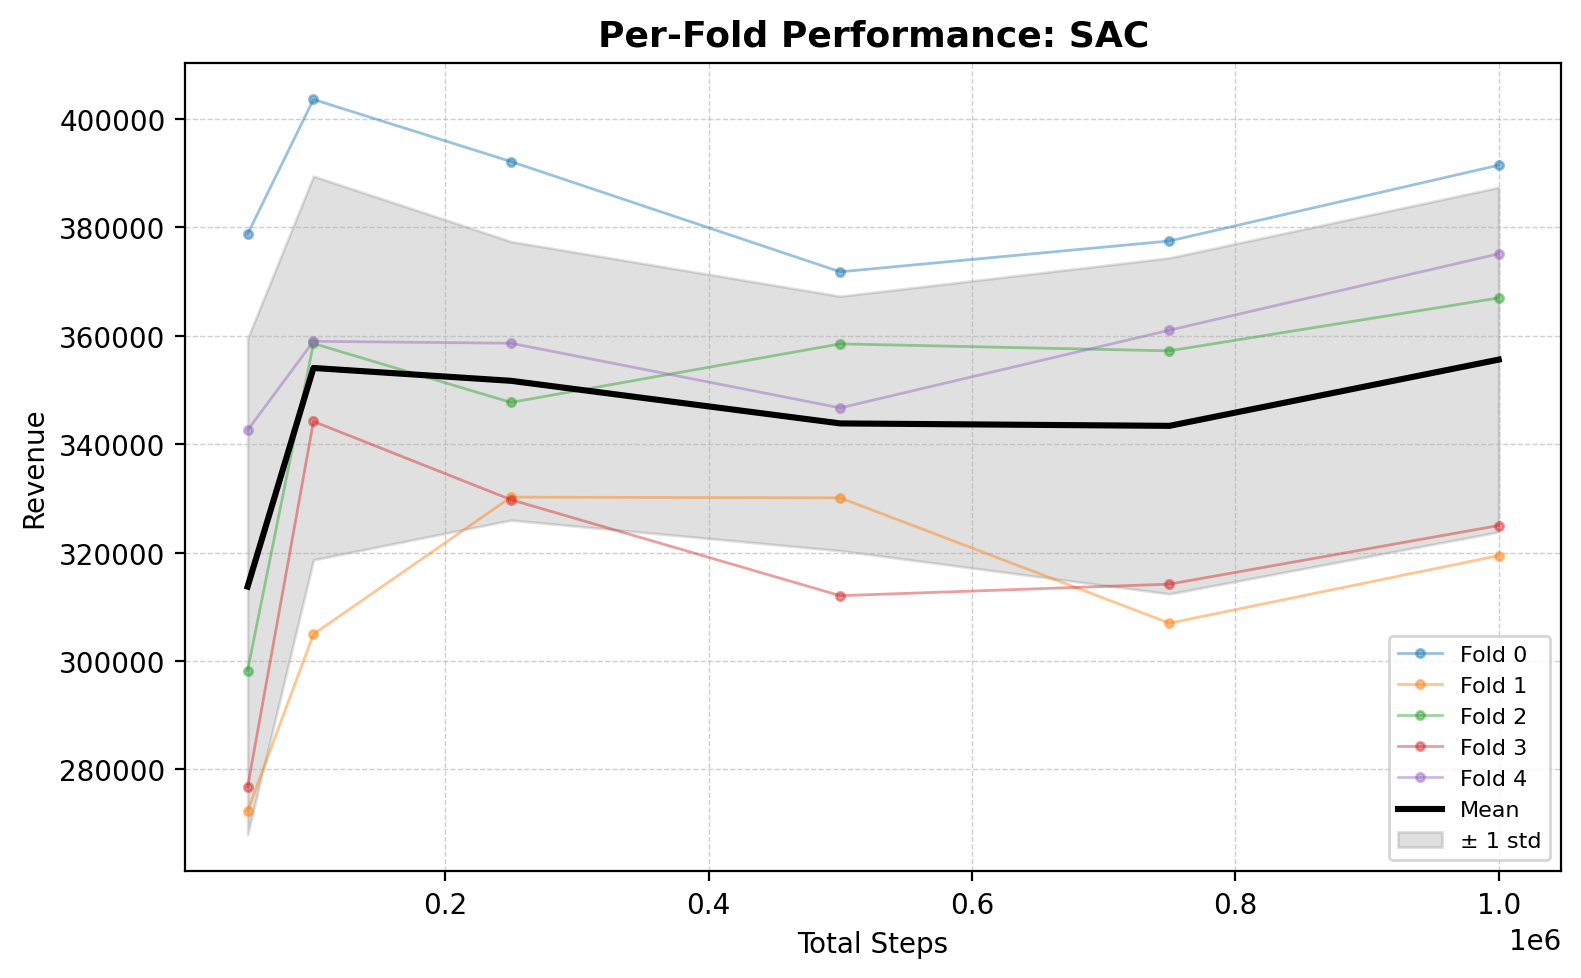
\includegraphics[width=\linewidth]{images/agent-evaluation/agent_per_fold_SAC.png}
                    \caption{Per-fold learning curves for the SAC agent, illustrating the mean net revenue and $\pm 1$ standard deviation across independent training runs.}
                    \label{fig:sac_per_fold}
                \end{minipage}\hfill
                \begin{minipage}{0.48\textwidth}
                    \centering
                    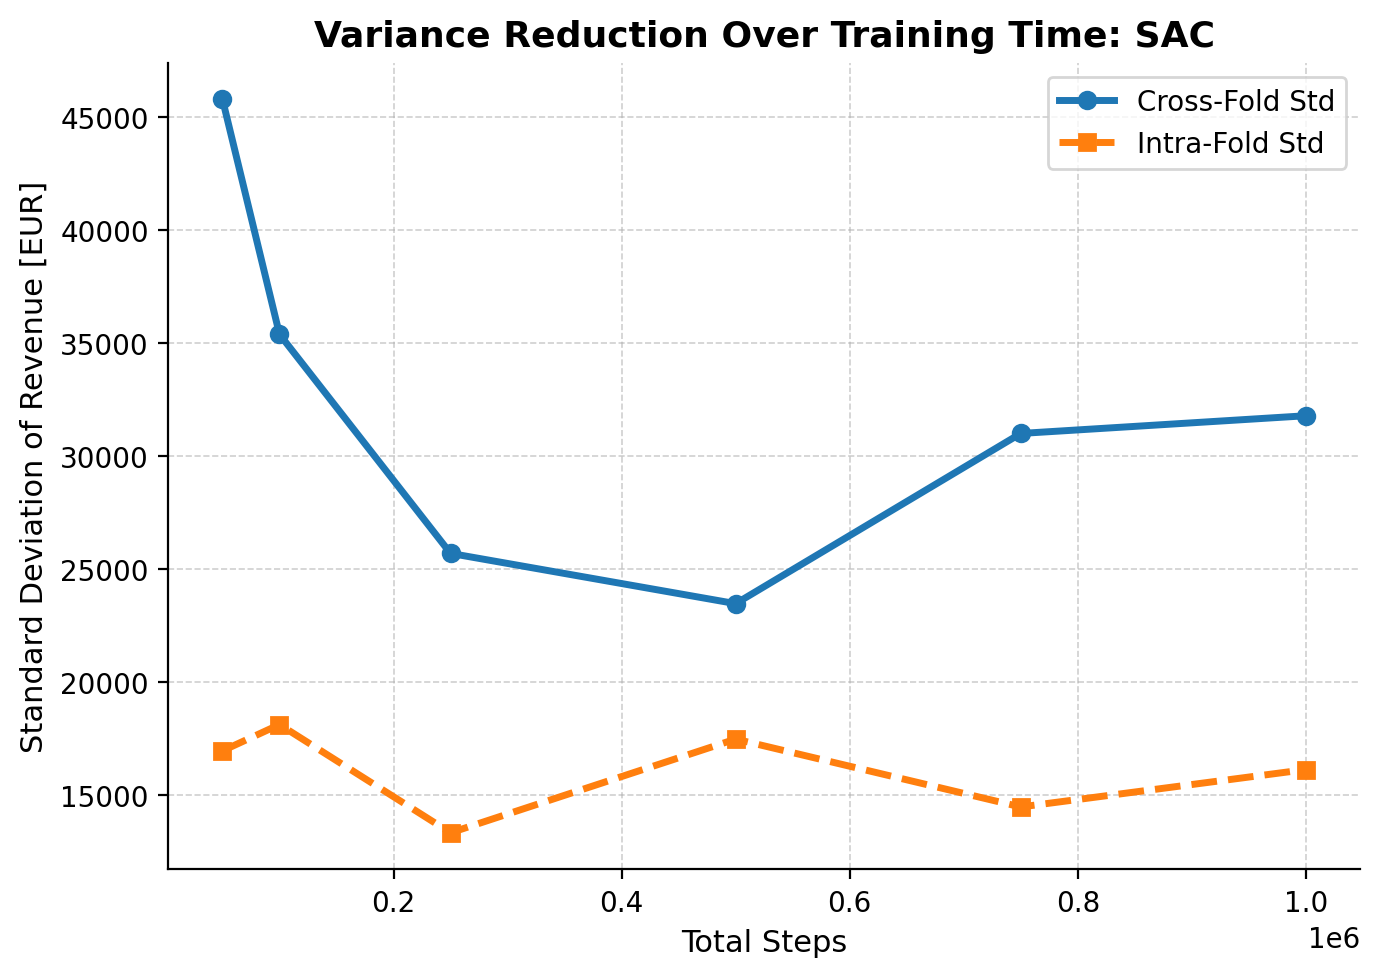
\includegraphics[width=\linewidth]{images/agent-evaluation/variance_over_time_SAC.png}
                    \caption{Comparison of Intra-Fold (Algorithmic) and Cross-Fold (Market) standard deviation for the SAC agent over the training horizon.}
                    \label{fig:sac_variance}
                \end{minipage}
            \end{figure}

            SAC exhibits a distinctive learning signature that reflects the interplay between its off-policy replay buffer and its entropy-driven exploration. The key observations are as follows:
            
            \begin{itemize}
                \item why it has a longer computation time

                \item Why it has almost instantly such a good result compared to the rest

                \item \textbf{Smoother cross-fold alignment:} Once the buffer reaches sufficient coverage, the mean revenue curves across all five folds converge tightly. The automatic entropy tuning ensures that each fold-specific run adapts its exploration intensity to the volatility of the local market regime encountered, rather than following a globally fixed schedule as in DQN's $\varepsilon$-greedy decay.

                \item 
                \textbf{Low and stable intra-fold variance:} Figure \ref{fig:sac_variance} shows that the Intra-Fold Standard Deviation of SAC remains consistently low. The dual-Q pessimism prevents any single run from being seduced by an overestimated Q-value into an erratic strategy, while the entropy bonus ensures that no run collapses prematurely to a degenerate policy. Together these mechanisms produce a high degree of algorithmic reproducibility across random seeds.

            \end{itemize}

            The maximum entropy framework therefore provides SAC with a natural hedge against the non-stationarity of the imbalance market: by remaining inherently exploratory, the agent avoids locking into patterns that were profitable in the training fold but fail to generalise to the shifted price dynamics of the test fold. This is particularly relevant in the context of the $hv$-block cross-validation, where each fold deliberately exposes the agent to all four seasons of price behaviour, and any overfit to one seasonal regime would be penalised across the remaining folds.


